\chapter{Asking Millionaires How They Got Rich (Austin)}

This chapter is not a blackboard lecture in the ordinary sense, but it does have a quantitative spine. We are led from one entrepreneur to the next by way of numbers---yearly earnings, daily profit spikes, revenue, capital raised, valuation, exit price, square footage, and assets under management---and then asked for the operating rule behind the number. The right way to read the episode is therefore to separate the categories of scale and then follow, in order, the mechanisms by which each guest claims to move from one scale to another.

\section{Cold Open: The Arithmetic of Wealth Claims}

The episode opens with a teaser montage. Its purpose is not yet explanation. It is to force several magnitudes into view so quickly that we feel the scale before we sort it. For the notes, the first act of discipline is bookkeeping: revenue, valuation, annual personal earnings, capital raised, and exit value are not the same object.

\begin{table}[h]
\centering
\begin{tabular}{|l|l|l|}
\hline
Symbol or category & Transcript claim & Interpretation \\
\hline
$R$ & $\approx \$30\,\text{million}$ & company revenue \\
$E_{\text{year}}$ & $\approx \$11.2\,\text{million}$ & personal annual earnings \\
$P_{\text{day,max}}$ & $\approx \$1\,\text{million}$ & peak daily take \\
$C_{\text{raised}}$ & $\approx \$87\,\text{million}$ & outside capital raised \\
$V$ & $\approx \$1\,\text{billion}$ & company valuation \\
$X$ & $\approx \$150\,\text{million}$, $\approx \$7\,\text{billion}$ & exit or deal value \\
$A_{\text{RE}}$ & hundreds of millions & assets under management \\
$V_{\text{RE,proj}}$ & $\approx \$2.5\,\text{billion}$ & projected developed value \\
\hline
\end{tabular}
\end{table}

This distinction matters immediately, because the montage is cut from later interviews. We are not yet in one argument. We are being given a map of the scales on which the later arguments will operate. Only after this does the host provide the governing frame: Austin is presented as a fast-growing city full of millionaires, and the city itself becomes the lecture hall.

\section{Josh: E-Commerce, Burst Profit, and Pricing Power}

The first sustained case is Josh. The structure is simple and deliberate. We begin with domain: e-commerce first, real estate second. We then move at once to magnitude:

\begin{align}
E_{\text{year}} &\approx \$11.2\,\text{million},\\
P_{\text{day,max}} &\approx \$1\,\text{million}.
\end{align}

The interesting claim is not merely that the numbers are large. It is that the distribution in time is uneven. Josh insists that it can be easier to make a great deal of money in a short window than to grind out a modest amount over a long one. The mechanisms he names are launches, promotions, joint ventures, holiday windows, and marketing strategy. If we want a compact mathematical proxy for that claim, we may write

\begin{equation}
v_P = \frac{\Delta P}{\Delta t},
\end{equation}

where $\Delta P$ is the profit captured in a campaign window $\Delta t$. This is not his formula; it is our clean way to express what he means by a higher ``velocity to profit.'' A business with ordinary daily flow can still have extraordinary intervals if the launch structure is right.

\subsection{Question \& Answer}

\paragraph{Question.} How can a business charge more and still grow?

\paragraph{Answer.} Josh's answer is to reject the false opposition between price and scale. He introduces the acronym WWAD, ``What Would Apple Do?'', and uses Apple as the model of a company that charges far above commodity competitors while continuing to dominate. The lecture's key maxim here is verbal rather than formal: price is only an issue when value is absent. The real variable is not price alone, but value relative to price.

What follows is pedagogically important. He does not celebrate originality for its own sake. He says, instead, that he bootstrapped by mimicking what already worked. In other words, the lecture pivots from the glamour of premium pricing to the sober discipline of studying an already successful premium operator.

This is the first major structural turn of the chapter. We move from scale as spectacle to value as mechanism.

\section{Josh's Operating System: Reviews, Delegation, and the 80/20 Rule}

Once the lecture has reframed price as a function of value, it asks the natural next question: how does one build value in a concrete business? Josh's answer is customer feedback. He speaks of taking reviews into a spreadsheet and dividing them by score:

\begin{equation}
\mathcal{R}_{\text{bad}} = \{1,2,3\}, \qquad
\mathcal{R}_{\text{good}} = \{4,5\}.
\end{equation}

This partition is the simplest formal object in the whole discussion, but it is useful. The higher reviews tell us what to preserve. The lower reviews tell us what customers resent, what they wish were present, and what can be improved. The method is not to guess at value. It is to let complaints specify the missing value.

\begin{figure}[h]
\centering
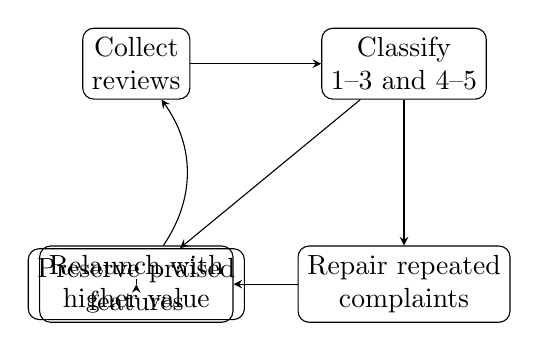
\begin{tikzpicture}[>=stealth, node distance=2.8cm]
\node[draw, rounded corners, align=center] (collect) {Collect\\reviews};
\node[draw, rounded corners, align=center, right of=collect, xshift=0.6cm] (classify) {Classify\\$1$--$3$ and $4$--$5$};
\node[draw, rounded corners, align=center, below of=classify] (repair) {Repair repeated\\complaints};
\node[draw, rounded corners, align=center, left of=repair, xshift=-0.6cm] (keep) {Preserve praised\\features};
\node[draw, rounded corners, align=center, below of=collect] (relaunch) {Relaunch with\\higher value};
\draw[->] (collect) -- (classify);
\draw[->] (classify) -- (repair);
\draw[->] (classify) -- (keep);
\draw[->] (keep) -- (relaunch);
\draw[->] (repair) -- (relaunch);
\draw[->] (relaunch) to[bend right=35] (collect);
\end{tikzpicture}

\smallskip
{\small A transcript-based reconstruction of Josh's review loop: preserve what customers already praise, repair what they repeatedly dislike, and relaunch the offer at a higher level of perceived value.}
\end{figure}

The same section introduces a second scaling principle. Josh recalls a line from a billionaire speaker: one need not answer a billion separate questions; one can answer one question that a billion people have. The move here is from individual transaction to shared pattern. A scalable business is not simply busier. It is attached to a broader recurring need.

Then the lecture turns again, from product logic to founder time. Josh says that his seven-to-eight-figure growth came from delegating MWA tasks---minimum wage activities---and concentrating on the small number of actions that truly moved the business. The 80/20 rule appears here not as a theorem but as a heuristic of concentration:

\begin{equation}
Y_{\text{high leverage}} \approx 0.8\,Y_{\text{total}}
\qquad \text{from} \qquad
X_{\text{key}} \approx 0.2\,X_{\text{activities}}.
\end{equation}

We should read this cautiously. The lecture is not proving a Pareto law. It is using the 80/20 language to insist that founder attention is a scarce variable, and that scale requires concentration rather than diffusion.

The host then resets the scene. Josh has supplied the episode's first dense operating model, and the lecture returns to downtown Austin in search of a different type of case.

\section{Bootstrapping, Loss Arithmetic, and Boring Compounding}

The next entrepreneur comes from residential and commercial solar. The shape of the argument changes. We are no longer in premium consumer e-commerce. We are in regional operating scale, expansion by sales channels, and bootstrapping from ordinary hustle: selling online, flipping sneakers, working early sales jobs, and building the company from scratch.

The metrics are concrete:

\begin{align}
R_{\text{now}} &\approx \$30\,\text{million},\\
R_{\text{target}} &\approx \$100\,\text{million}.
\end{align}

The target is stated on a two-to-three-year horizon, which means the lecture is now mixing current scale with projected scale. Again, bookkeeping matters.

\subsection{Question \& Answer}

\paragraph{Question.} Why does boring compounding beat flashy wins?

\paragraph{Answer.} The answer begins with loss arithmetic. The speaker quotes Buffett's rule not to lose money, then gives the key example: if we lose $50\%$, we do not need a $50\%$ gain to recover. We need a $100\%$ gain. Let us write that carefully.

Suppose wealth falls from $W_0$ to
\begin{equation}
W_1 = (1-L)W_0,
\end{equation}
where $L$ is the fractional loss. To recover, we need a gain fraction $g$ satisfying
\begin{equation}
W_1(1+g) = W_0.
\end{equation}
Solving for $g$, we get
\begin{align}
g &= \frac{W_0-W_1}{W_1}\\
  &= \frac{L}{1-L}.
\end{align}

\paragraph{Worked example.} If $L=0.5$, then
\begin{equation}
g = \frac{0.5}{0.5} = 1 = 100\%.
\end{equation}

This is the cleanest explicit derivation in the lecture. Its force is practical: deep losses destroy compounding because recovery demands disproportionately large later gains.

The speaker then turns from avoiding losses to accumulating steadily. He cites a rough annual return band of eight to ten percent and recommends automating money into index funds. In the simplest reconstruction, if returns compound at annual rate $r$, then

\begin{equation}
r \in [0.08,\,0.10],
\end{equation}
and pure compounding takes the form
\begin{equation}
W_n = W_0(1+r)^n.
\end{equation}

With a fixed annual contribution $c$, the standard update becomes
\begin{equation}
W_n = W_0(1+r)^n + c\,\frac{(1+r)^n-1}{r}.
\end{equation}

The lecture calls the visible late steepening a ``J curve.'' We should interpret that modestly: not as a technical private-equity object, but as the ordinary visual acceleration of compounding when gains themselves begin to earn gains.

\begin{figure}[h]
\centering
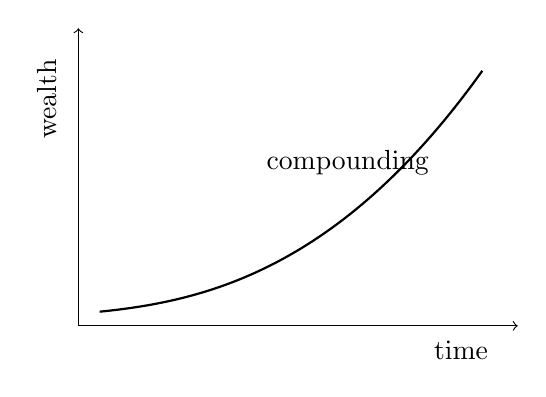
\begin{tikzpicture}[scale=0.9]
\draw[->] (0,0) -- (6.2,0);
\draw[->] (0,0) -- (0,4.2);
\draw[thick] (0.3,0.2) .. controls (1.8,0.35) and (3.7,0.8) .. (5.7,3.6);
\node at (5.4,-0.35) {time};
\node[rotate=90] at (-0.45,3.2) {wealth};
\node at (3.8,2.3) {compounding};
\end{tikzpicture}

\smallskip
{\small A schematic version of the compounding picture invoked in the interview: the early years seem nearly flat, while the later years rise sharply enough to change the scale of the result.}
\end{figure}

What follows is not an abstract investment lecture. It is a blueprint: work on oneself, pick something boring and become excellent at it, scale the craft, then move the proceeds into appreciating assets that can compound. The examples of plumbing, roofing, and flooring matter because they strip glamour out of the equation. The point is mastery and repetition, not novelty.

\section{Commercial Real Estate: Scale, Index Funds, and Alignment}

The next major case is Ari in commercial real estate. The lecture now shifts from bootstrapped operating growth to institutional scale. We are given several different magnitudes, and they must not be merged carelessly:

\begin{align}
A_{\text{RE}} &\sim \text{hundreds of millions of dollars},\\
S_{\text{construction}} &> 10^6\ \text{ft}^2,\\
S_{\text{Tesla}} &\approx 600{,}000\ \text{ft}^2,\\
V_{\text{projected}} &\approx \$2.5\,\text{billion}.
\end{align}

These are different measures: current assets under management, current square footage under construction, one specific nearby project, and a later projected developed value. The lecture uses them to convey scale, not to propose a single balance-sheet identity.

Ari then gives advice that drops almost all the glamour of real estate. How should ordinary money be made to work? Index funds, broad equity exposure, and automated contributions. In that sense, this section loops back to the previous one: the proper use of surplus is compounding, not restless activity.

But Ari's most distinctive contribution is on sales. He says, in effect, that the client in real estate is not merely seeking return; the client is trying not to be fooled. The hidden variable is fear. Risk control, demonstrated care, invested personal capital, and aligned interests reduce that fear. Schematically, his distinction is this:

\begin{equation}
\text{manager payoff} \propto \text{performance}
\qquad \text{rather than} \qquad
\text{manager payoff} \propto \text{capital raised}.
\end{equation}

This is a stylized reconstruction, but it captures the logic of his contrast between the fee business and the performance business. Once incentives are aligned, trust ceases to be a vague moral word and becomes part of the sales mechanism itself.

The host then resets again. We have moved from consumer value to operating scale to institutional trust. The next pivot is into venture-backed technology.

\section{Technology Startups: Product, Team, and Funding}

Renji's case changes the language of scale. He is in AR, VR, spatial computing, software, and hardware. The quantities here belong to the world of venture and multiples:

\begin{align}
C_{\text{raised}} &\approx \$87\,\text{million},\\
V &\approx \$1\,\text{billion}.
\end{align}

The lecture is careful, and our notes must be even more careful: valuation is not revenue. In symbols,

\begin{equation}
V \neq R.
\end{equation}

That distinction is crucial because the host asks how much the business will ``generate,'' while the answer immediately shifts into valuation. The explanation is that technology companies often command higher multiples than ordinary operating businesses. So the lecture moves from arithmetic into market structure.

\subsection{Question \& Answer}

\paragraph{Question.} What is the blueprint for a startup that survives and scales?

\paragraph{Answer.} Renji gives a three-part sequence, and it is worth preserving almost as a theorem schema for startups:

\begin{enumerate}
\item Build a product that people actually want.
\item Build the team that can build and improve that product.
\item Secure the funding, or the internally generated cash flow, that keeps the team alive long enough to scale.
\end{enumerate}

This is the startup version of the lecture's recurring refusal of fantasy. It is not enough to enter a fashionable sector. One must differentiate. Renji explicitly criticizes the tendency to jump into whatever seems to be making money merely because it is already being done by others. The lecture therefore ends this section by tightening the relation between demand, capability, and financing. Valuation is the effect of that triangle, not the starting point.

\section{The Anti-Myth Ending}

The final founder functions as a corrective. He tells a story of ending up in high tech almost against his earlier inclinations, then co-founding companies in Austin, selling one for about $\$150$ million, participating in a later go-private round of about $\$7$ billion, and helping build a company with more than half a billion in revenue and roughly $2{,}500$ employees.

\begin{align}
X_{\text{first exit}} &\approx \$150\,\text{million},\\
X_{\text{go-private}} &\approx \$7\,\text{billion},\\
R_{\text{later company}} &> \$0.5\,\text{billion}.
\end{align}

Yet the lecture does not let these numbers stand as the final lesson. Instead, it moves against the mythology of the solitary genius. His advice is twofold: know what you are good at, and surround yourself with people who are strong where you are weak. His account of scaling goes further: the famous founders are almost always remembered as isolated heroes, but in reality they were enabled by one or several key collaborators. Teams, not myths, carry businesses to very large scale.

This is a fitting end. The episode began with a barrage of gigantic numbers. It ends by insisting that those numbers are the surface of a much more ordinary truth: self-knowledge, complementarity, and institutional structure matter more than heroic self-image.

\section{Summary}

We can now see the architecture of the lecture clearly. It begins with the arithmetic of wealth claims and then, case by case, translates numbers into mechanisms. Josh gives the logic of premium pricing, imitation of what already works, review-driven improvement, and concentrated founder attention. The solar entrepreneur gives the arithmetic of avoiding loss, the discipline of compounding, and the dignity of boring mastery. Ari adds institutional trust, index-fund simplicity, and incentive alignment. Renji supplies the startup triangle of product, team, and funding. The final founder removes the last illusion by denying that scale is a solo performance.

If we compress the whole episode to one line, it is this: wealth is not one number, and scale is not one trick. The lecture teaches us to distinguish the measures, identify the mechanism appropriate to each measure, and then follow the long chain by which money is earned, preserved, reinvested, and organized through other people.